% Esta sección describe equipo y procedimiento de manera simple.
% Reemplaza con tu propio contenido cuando enseñes o evalúes.

\subsection{Actividad 1} % Sub-sección (nivel bajo \section) para detallar hardware

\subsubsection{Caso de estudio}

Se desea diseñar un sistema basado en microcontrolador que:
\begin{itemize}
    \item Lea un sensor cada 10 ms.
    \item Controle un motor según la lectura.
    \item Envíe datos por comunicación serial cada 100 ms.
    \item Atienda un botón de emergencia que debe detener todo inmediatamente.
    \item Muestre información en una pantalla.
\end{itemize}
\vspace{0.3cm}
\begin{itemize}
    \item\textbf{ ¿Cómo implementar esto usando solo un while?:}
    La respuesta de esta pregunta genera como resultado el diagrama de flujo que se encuentra en la figura \ref{Diagrama de flujo}.
     
    \vspace{0.3cm}
    \item \textbf{¿Qué problemas podrían aparecer?:} Al ser un while con dependencia doble, interna y distinta del tiempo; se puede estar presentando retrasos de lectura, pues la lectura lineal debe esperar a, por ejemplo, enviar el paquete de datos por el puerto serial para continuar con el proceso. Esto mismo trae problemas de latencia y de estabilidad, pues en el caso que se desee agregar mas tareas, el control del tiempo se verá aún mas afectado.
    \vspace{0.3cm}
    \item \textbf{¿Qué tarea sería más crítica?:} En este caso desarrollado, se entiende que la tarea más critica seria toda la que conlleve al botón de emergencia, pues estamos hablando de factores de seguridad humana y estos deben ser considerados de manera prioritaria.
    \vspace{0.3cm}
    \item \textbf{¿Cómo garantizarías tiempos de respuesta?:} En una primera parte, se deberían independizar dos elementos claves: La parada de emergencia y el timer, pues estos deben ser independientes de una revisión ocasional dentro del while. Una manera de hacerlo es generando interrupciones; asegurando una baja latencia y por lo tanto (en el caso de la parada de emergencia) un menor tiempo de reacción. Por parte del Timer; considero que se debería tratar como variable independiente donde dicha variable sea la única que gestione la lectura y el envío de datos con el fin de asegurar un "espacio de memoria" que realmente cumpla los tiempos establecidos.
\end{itemize}
\begin{figure}
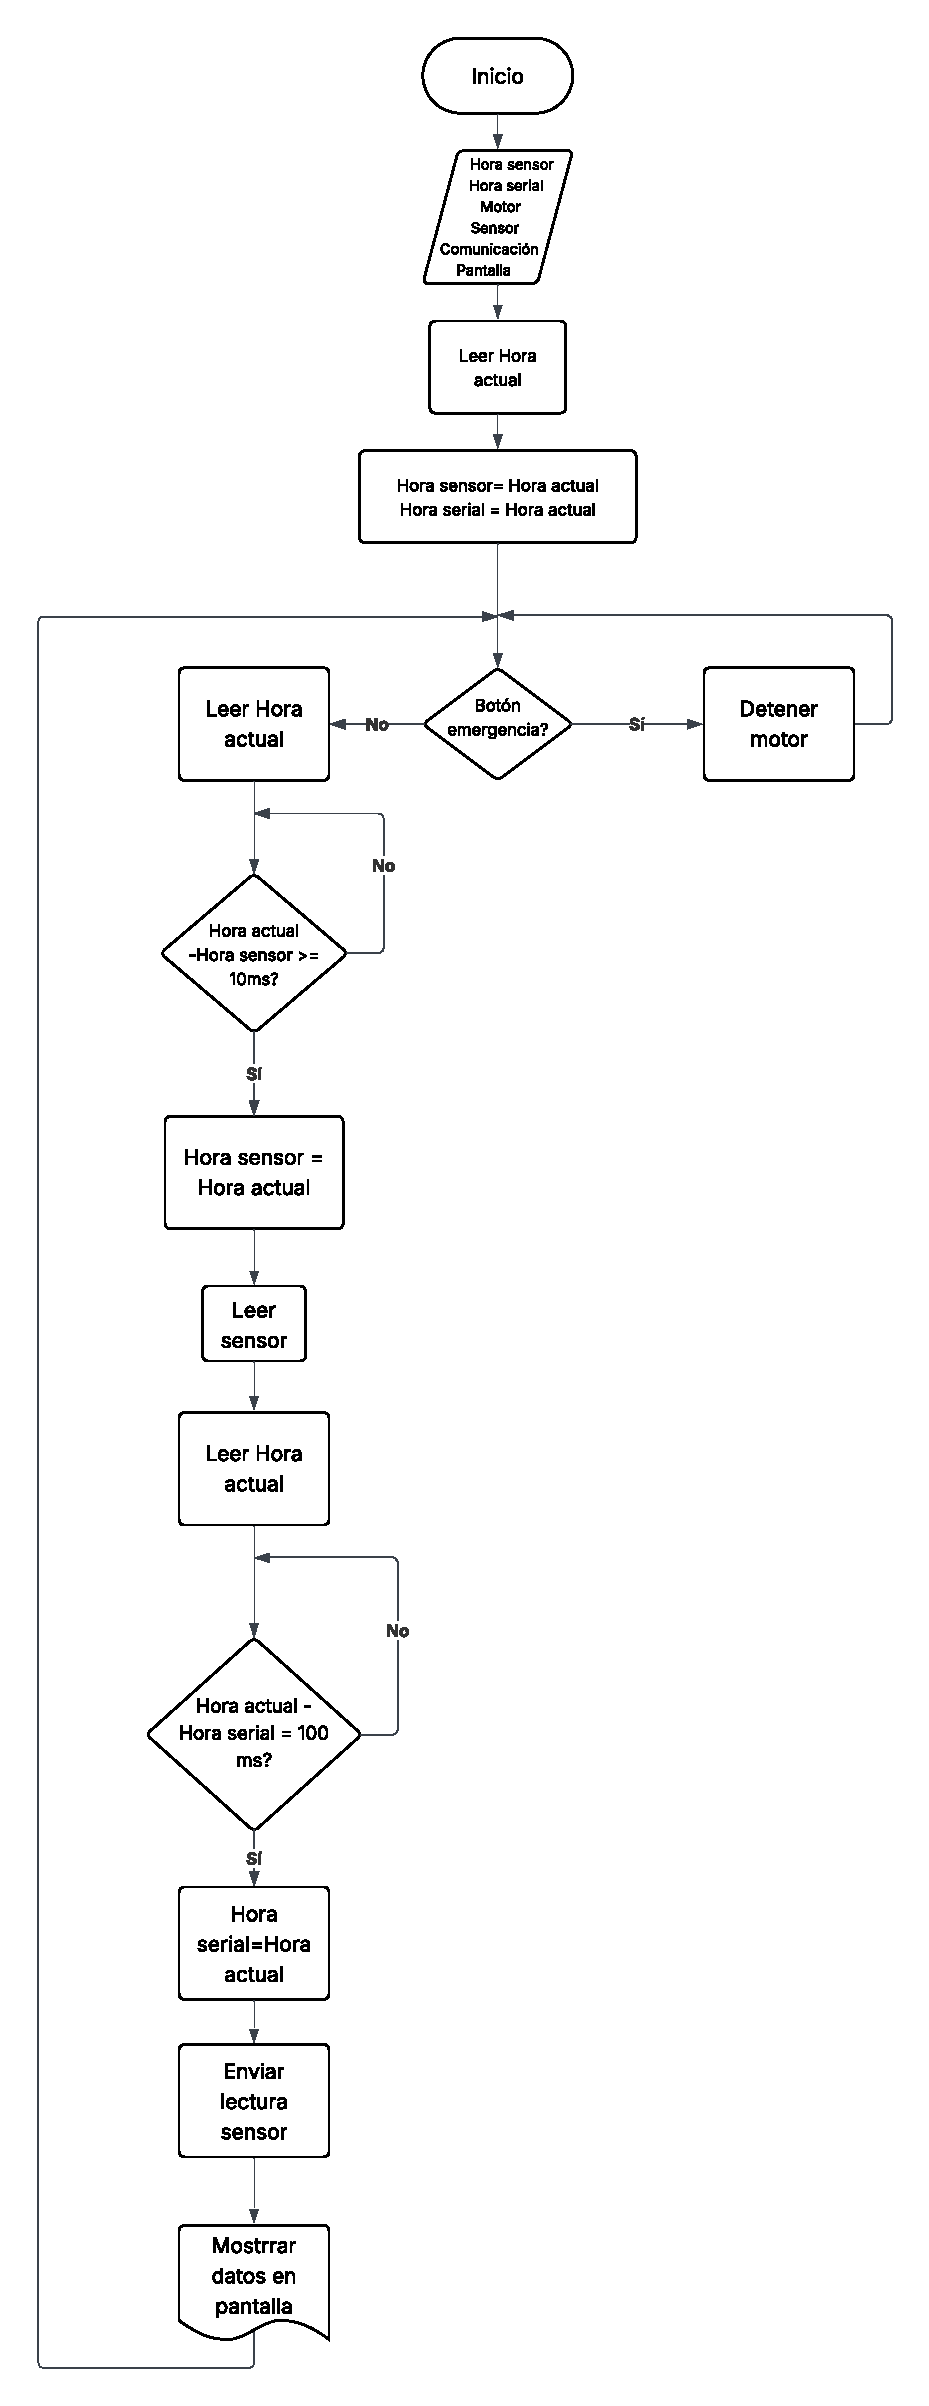
\includegraphics[width=0.4\textwidth]{images/Diagramawhile.pdf}
\caption{Diagrama de flujo de la implementación del while} % Texto bajo la figura
  \label{Diagrama de flujo}          % Etiqueta para referenciar con \ref{fig:res_fig}
\end{figure}
\vspace{0.3cm}
\subsubsection{Trabajo de consulta}
\begin{itemize}
    \item \textbf{Interrupciones:} Las interrupciones son mecanismos que permiten a un microcontrolador suspender temporalmente la ejecución del programa para atender un evento inmediato. Cuando ocurre dicho evento, el hardware guarda el estado del procesador, ejecuta una Rutina de Servicio de Interrupción (\textit{Interrupt Service Routine}-ISR) y luego restaura el estado para continuar la ejecución normal.\\
    Su función principal es evitar el \textit{polling} (método en el que el procesador revisa continuamente si ocurrió un evento, en lugar de esperar a que una interrupción lo notifique) constante y mejorar el tiempo de respuesta ante eventos internos o externos, siendo esenciales en sistemas de tiempo real. \cite{valvano2011embedded} No obstante, pueden generar condiciones de carrera, aumento de latencia si la ISR es extensa y problemas de memoria de pila, por lo que deben implementarse de forma breve y controlada. \cite{buttazzo1997hard}   
    \vspace{0.3cm}
    \item \textbf{Planificación y Scheduler:}  El scheduler (planificador) es el componente del sistema operativo o del software de control que decide qué tarea se ejecuta y en qué momento. En sistemas embebidos con multitarea, su función es administrar el uso del procesador cuando existen varias tareas que requieren ejecución, garantizando orden y control en el acceso al CPU (\textit{Central Processing Unit}).\cite{buttazzo1997hard}
    La prioridad es el nivel de importancia asignado a cada tarea. Determina cuál debe ejecutarse primero cuando varias están listas al mismo tiempo... Una tarea con mayor prioridad desplaza a otra de menor prioridad si el sistema lo permite.
    La planificación preventiva (preemptiva) es aquella en la que el scheduler puede interrumpir una tarea en ejecución para asignar el procesador a otra de mayor prioridad. En cambio, la planificación cooperativa requiere que la tarea en ejecución ceda voluntariamente el control del procesador, por lo que el cambio de tarea ocurre solo cuando esta finaliza o libera el CPU. \cite{buttazzo1997hard}
    \vspace{0.3cm}
    \item \textbf{Multitarea:} La concurrencia es la capacidad de un sistema para gestionar múltiples tareas que progresan en intervalos de tiempo superpuestos. No implica necesariamente que todas se ejecuten exactamente al mismo tiempo, sino que el sistema organiza su ejecución de manera que todas avancen sin bloquearse mutuamente.\cite{buttazzo1997hard}
    La multitarea real ocurre cuando varias tareas se ejecutan simultáneamente en diferentes núcleos de procesamiento. En cambio, la multitarea simulada se presenta en sistemas con un solo núcleo, donde el procesador alterna rápidamente entre tareas mediante un scheduler, dando la impresión de ejecución simultánea aunque solo una tarea se ejecuta en cada instante.\\
    En sistemas embebidos, ejemplos de multitarea incluyen: un microcontrolador que controla un motor mientras lee sensores y transmite datos por comunicación serial; un sistema IoT (\textit{Internet of Things}) que adquiere datos, los procesa y los envía a la nube; o un dispositivo médico que monitorea señales mientras actualiza una pantalla. En todos estos casos, las tareas comparten el procesador y requieren coordinación adecuada. \cite{valvano2011embedded}
     \vspace{0.3cm}
    \item \textbf{Sincronización: } Una condición de carrera es una situación que ocurre cuando dos o más tareas acceden y modifican un mismo recurso o variable compartida de manera simultánea, y el resultado final depende del orden impredecible en que se ejecuten \cite{buttazzo1997hard}. Esto puede generar inconsistencias o corrupción de datos si no existen mecanismos de control adecuados.\\
    Los semáforos y los mutex son mecanismos de sincronización utilizados para coordinar el acceso a recursos compartidos. Un semáforo es una variable de control que regula la disponibilidad de un recurso y puede permitir uno o varios accesos según su tipo. Un mutex (mutual exclusion) es un mecanismo específico que garantiza que solo una tarea a la vez pueda acceder a un recurso, asegurando exclusión mutua.\\
    Una sección crítica es el fragmento de código en el que se accede a un recurso compartido y que, por lo tanto, debe ejecutarse de forma exclusiva para evitar interferencias entre tareas. Para protegerla, se emplean mecanismos como mutex, semáforos o des-habilitación temporal de interrupciones. \cite{valvano2011embedded}
\end{itemize}

\input{tables/table1a.tex}   % Inserta el archivo de tabla (lista de equipos) en este punto


